
%Part 21: Lazy is as Lazy Doesn’t: Twisted and Haskell
\section{Twisted и Haskell\label{sec:part21}}

\subsection{Введение}

%In the last Part we compared Twisted with Erlang, giving most of our attention to some ideas they have in common. And that ended up being pretty simple, as asynchronous I/O and reactive programming are key components of the Erlang runtime and process model.
В предыдущей главе мы сравнивали Twisted с Erlang'ом, 
уделяя внимание некоторым идеям, являющимися для них общими. 
В результате все оказалось достаточно простым, поскольку 
асинхронный ввод-вывод и реативное программирование - 
ключевые компоненты среды и модели процесса Erlang.


%Today we are going to range further afield and look at Haskell, another functional language that is nevertheless quite different from Erlang (and, of course, Python). There won’t be as many parallels, but we will nevertheless find some asynchronous I/O hiding under the covers.
Сегодня мы собираемся побродить вдалеке и посмотреть на 
\href{http://haskell.org/}{Haskell}\footnote[1]{http://haskell.org/}, 
еще один функциональный язык, который отличается от Erlang'а (и, конечно, от Python'а). 
Здесь не будет так много сходств, но мы, тем не менее, найдем 
спрятый под оболочкой асинхронный ввод-вывод. 


%Functional with a Capital F
\subsection{Функциональность с заглавной Ф}

%Although Erlang is also a functional language, its main focus is a reliable concurrency model. Haskell, on the other hand, is functional through and through, making unabashed use of concepts from category theory like functors and monads.
Хотя Erlang также является функциональным языком, он в основном 
сфокусирован на надежной модели согласованности. Haskell наоборот - 
функциональный во всех отношениях, что делает его неотъемлемой 
частью концепции \href{http://en.wikipedia.org/wiki/Category\_theory}{теории категорий}\footnote[2]{http://en.wikipedia.org/wiki/Category\_theory},  
подобной \href{http://en.wikipedia.org/wiki/Functor}{функторам}\footnote[3]{http://en.wikipedia.org/wiki/Functor} 
и \href{http://en.wikipedia.org/wiki/Monad\_\%28category\_theory\%29}{монадам}\footnote[4]{http://en.wikipedia.org/wiki/Monad\_\%28category\_theory\%29}.


%Don’t worry, we’re not going into any of that here (as if we could). Instead we’ll focus on one of Haskell’s more traditionally functional features: laziness. Like many functional languages (but unlike Erlang), Haskell supports lazy evaluation. In a lazily evaluated language the text of a program doesn’t so much describe how to compute something as what to compute. The details of actually performing the computation are generally left to the compiler and runtime system.
Не беспокойтесь, мы не собираемся сейчас в это погружаться. 
Вместо этого мы сфокусируемся на одной наиболее 
традиционной функциональной особенности: ленивости. Подобно 
большинству функциональных языков (но в отличии от Erlang'а), Haskell 
поддерживает \href{http://en.wikipedia.org/wiki/Lazy\_evaluation}{ленивые вычисления}\footnote[5]{http://en.wikipedia.org/wiki/Lazy\_evaluation}. 
В языке ленивых вычислений текст программы не описывает то как 
что-то вычислять, а больше - что вычислять. Детали действительной 
обработки вычислений обычно скрываются за компилятором и исполняющей системой.


%And, more to the point, as a lazily-evaluated computation proceeds the runtime may evaluate expressions only partially (lazily) instead of all at once. In general, the runtime will evaluate only as much of an expression as is needed to make progress on the current computation.
И, нужно отметить, что по мере обработки ленивых вычислений, 
исполняющая система может вычислять выражения только частично (лениво), 
а не полностью. В целом, исполняющая система обрабатывает так много от 
выражения, сколько нужно для того, чтобы сдвинуться в текущих вычислениях. 


%Here is a simple Haskell statement applying head, a function that retrieves the first element of a list, to the list [1,2,3] (Haskell and Python share some of their list syntax):
Далее простой оператор Haskell'а, применяющий 
функцию \textit{head}, которая получает первый элемент из списка \textit{[1,2,3]} (Haskell и 
Python имеют общий синтаксис для списка): 

\begin{scriptsize}\begin{verbatim}
  head [1,2,3]
\end{verbatim}\end{scriptsize}


%If you install the GHC Haskell runtime, you can try this out yourself:
Если вы установили среду исполнения 
\href{http://www.haskell.org/ghc/}{GHC Haskell}, вы можете 
попробовать это сами:

\begin{scriptsize}\begin{verbatim}
[~] ghci
GHCi, version 6.12.1: http://www.haskell.org/ghc/  : ? for help
Loading package ghc-prim ... linking ... done.
Loading package integer-gmp ... linking ... done.
Loading package base ... linking ... done.
Prelude> head [1,2,3]
1
Prelude>
\end{verbatim}\end{scriptsize}


%The result is the number 1, as expected.
Результат, как и ожидалось, - число 1.


%The Haskell list syntax includes the handy ability to define a list from its first couple of elements. For example, the list [2,4 ..] is the sequence of even numbers starting with 2. Where does it end? Well, it doesn’t. The Haskell list [2,4 ..] and others like it represent (conceptually) infinite lists. You can see this if you try to evaluate one at the interactive Haskell prompt, which will attempt to print out the result of your expression:
Синтаксис списка в Haskell имеет удобное свойство определять 
список через свои первые несколько аргументов. Например, 
список [2,4 ..] - последовательность четных чисел, начинающихся с 2. 
Где же конец? А его и нет. В Haskell список [2,4 ..] и другие подобные 
представляют (концептуально) бесконечные списки.   


\begin{scriptsize}\begin{verbatim}
Prelude> [2,4 ..]
[2,4,6,8,10,12,14,16,18,20,22,24,26,28,30,
32,34,36,38,40,42,44,46,48,50,52,54,56,58,
60,62,64,66,68,70,72,74,76,78,80,82,84,86,
88,90,92,94,96,98,100,102,104,106,108,110,
...
\end{verbatim}\end{scriptsize}


%You'll have to press Ctrl-C to stop that computation as it will never actually terminate. But because of lazy evaluation, it is possible to use these infinite lists in Haskell with no trouble:
Вы должны нажать Ctrl-C для того, чтобы остановить вычисление, так 
как оно само не завершится. Ввиду ленивости вычислений, то можно без проблем 
использовать эти бесконечные циклы в Haskell:

\begin{scriptsize}\begin{verbatim}
Prelude> head [2,4 ..]
2
Prelude> head (tail [2,4 ..])
4
Prelude> head (tail (tail [2,4 ..]))
6
\end{verbatim}\end{scriptsize}


%Here we are accessing the first, second, and third elements of this infinite list respectively, with no infinite loop anywhere in sight. This is the essence of lazy evaluation. Instead of first evaluating the entire list (which would cause an infinite loop) and then giving that list to the head function, the Haskell runtime only constructs as much of the list as it needs for head to finish its work. The rest of the list is never constructed at all, because it is not needed to proceed with the computation.
Здесь мы сначала берем соответственно первый, второй и третий элементы бесконечного 
списка без бесконечного зацикливания. В этом  и есть сущность ленивых вычислений. 
Вместо того, чтобы сначада вычислить весь список (который может привести к 
бесконечному циклу), и затем дать этот список функции head, исполняющая система Haskell 
только конструирует столько элементов в списке, сколько нужно для того, чтобы 
head завершила свою работу. Остальные элементы в списке никогда не конструируются, 
поскольку вычисления не нужно продолжать.   


%When we bring the tail function into play, Haskell is forced to construct the list further, but again only as much as it needs to evaluate the next step of the computation. And once the computation is done, the (unfinished) list can be discarded.
Когда мы вводим в игру функцию tail, то Haskell вынужден 
продолжить создание списка, но снова только до того момента, когда 
достаточно для вычисления следующего шага. И как только вычисления 
сделаны, (незаконченный) список может быть сброшен.  


%Here’s some Haskell code that partially consumes three different infinite lists:
Далее некоторый код на Haskell, который частично отбрасывает три 
различных бесконечных списка: 

\begin{scriptsize}\begin{verbatim}
Prelude> let x = [1..]
Prelude> let y = [2,4 ..]
Prelude> let z = [3,6 ..]
Prelude> head (tail (tail (zip3 x y z)))
(3,6,9)
\end{verbatim}\end{scriptsize}


%Here we zip all the lists together, then grab the head of the tail of the tail. Once again, Haskell has no trouble with this and only constructs as much of each list as it needs to finish evaluating our code. We can visualize the Haskell runtime “consuming” these infinite lists in Figure 46:
Здесь мы соединяем все списки, затем берем голову хвоста от хвоста. 
И снова, Haskell не имеет с этим проблем и только конструирует 
столько элементов в списке, сколько нужно, чтобы 
завершить выполнение вашего кода. Мы можем визуализировать 
исполняющую среду Haskell'а <<потребляющую>> эти бесконечные списки на рисунке \ref{fig:haskell}:  

% fig46
\begin{figure}[h]
\begin{center}
    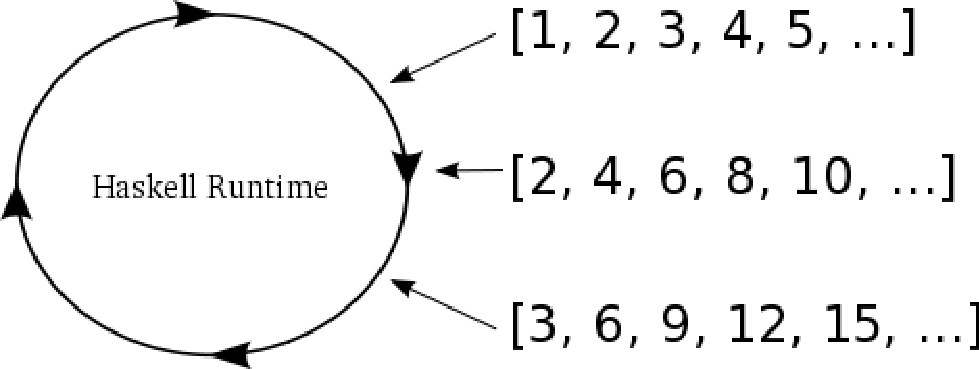
\includegraphics[width=0.5\textwidth]{images/haskell.pdf}
    \caption{Haskell, потребляющий некоторые бесконечные списки\label{fig:haskell}}
\end{center}
\end{figure}

%Although we’ve drawn the Haskell runtime as a simple loop, it might be implemented with multiple threads (and probably is if you are using the GHC version of Haskell). But the main point to notice is how this figure looks like a reactor loop consuming bits of data as they come in on network sockets.
Хотя мы изобразили исполняющую среду Haskell как простой цикл, 
он мог бы быть реализован несколькими потоками (и, вероятно, это 
так и есть, если вы используете GHC версию Haskell). Но основная 
мысль, в том, что рисунок выглядит как реакторный цикл, 
потребляющий данных по мере их поступления на сетевые сокеты.   


%You can think of asynchronous I/O and the reactor pattern as a very limited form of lazy evaluation. The asynchronous I/O motto is: “Only process as much data as you have”. And the lazy evaluation motto is: “Only process as much data as you need”. Furthermore, a lazily-evaluated language applies that motto almost everywhere, not just in the limited scope of I/O.
Выможете думать об асинхронном вводе-выводе и 
реакторном шаблоне как об очень ограниченной 
форме ленивых вычислений. Лозунг асинхронного программирования: 
"Обработать столько данных, сколько имеется". А лозунг 
ленивых вычислений: "Обработать столько данных, сколько нужно". 
Более того, язык ленивых вычислений применяет этот лозунг 
практически везде, не ограничиваясь только вводом-выводом.


%But the point is that, for a lazily-evaluated language, making use of asynchronous I/O is no big deal. The compiler and runtime are already designed to process data structures bit by bit, so lazily processing the incoming chunks of an I/O stream is just par for the course. And thus the Haskell runtime, like the Erlang runtime, simply incorporates asynchronous I/O as part of its socket abstractions. And we can show that by implementing a poetry client in Haskell.
Но основная мысль в том, что язык ленивых вычислений позволяет 
несложно реализовывать асинхронный ввод-вывод. 

Компилятор и 
исполняющая среда уже спроектированы так, чтобы обрабатывать 
структуры данных бит за битом, что равносильно ленивой обработке  
приходящих кусков асинхронного потока. 


И таким образом исполняющая среда Haskell, подобно исполняющей 
среде Erlang, просто включает асинхронный ввод-вывод как часть 
своих сокетных абстракций. И мы можем продемонстрировать это, 
реализуя поэтический клиент на Haskell.


\subsection{Haskell поэзия}


%Our first Haskell poetry client is located in haskell-client-1/get-poetry.hs. As with Erlang, we’re going to jump straight to a finished client, and then suggest further reading if you’d like to learn more.
Наш первый поэтический клиент на Haskell'е расположен в 
\href{https://github.com/jdavisp3/twisted-intro/blob/master/haskell-client-1/get-poetry.hs}{haskell-client-1/get-poetry.hs}. 
Также как и с Erlang, мы собираемся сразу же перейти к окончательной версии 
клиента, и затем предложить ссылки для дополнительного чтения, если вы 
хотите изучить больше.


%Haskell also supports light-weight threads or processes, though they aren’t as central to Haskell as they are to Erlang, and our Haskell client creates one process for each poem we want to download. The key function there is runTask which connects to a socket and starts the getPoetry function in a light-weight thread.
Haskell также поддерживает легковесные потоки и процессы, хотя 
они не являются центральным местом в Haskell, в отличие от Erlang, 
и наши Haskell клиенты создают один процесс для каждой 
поэмы, которую мы хотим выкачать. Ключевая функция здесь - это 
\href{https://github.com/jdavisp3/twisted-intro/blob/master/haskell-client-1/get-poetry.hs#L64}{runTask}, 
которая соединяется с сокетом и запускает функцию 
\href{https://github.com/jdavisp3/twisted-intro/blob/master/haskell-client-1/get-poetry.hs#L48}{getPoetry} 
в легковесном потоке.


%You’ll notice a lot of type declarations in this code. Haskell, unlike Python or Erlang, is statically typed. We don’t declare types for each and every variable because Haskell will automatically infer types not explicitly declared (or report an error if it can’t). A number of the functions include the IO type (technically a monad) because Haskell requires us to cleanly separate code with side-effects (i.e., code that performs I/O) from pure functions.
В коде вы обнаружите много объявлений типов. Haskell, в отличие от Python'а  
или Erlang'а, ститически типизированный. Мы не объявляем тип для каждой 
переменной, потому что Haskell автоматически определяет типы для неявно 
определенных переменных (или сообщает ошибку, если он не может определить). 
Ряд функций включает тип IO (технически это монада), поскольку Haskell 
требует от нас четко разделять код со сторонними эффектами (например, 
код, выполняющий ввод-вывод) от чистых функций.


%The getPoetry function includes this line:
Функция \textit{getPoetry} включает следующую строчку:

\begin{scriptsize}\begin{verbatim}
poem <- hGetContents h
\end{verbatim}\end{scriptsize}


%which appears to be reading the entire poem from the handle (i.e., the TCP socket) at once. But Haskell, as usual, is lazy. And the Haskell runtime includes one or more actual threads which perform asynchronous I/O in a select loop, thus preserving the possibilities for lazy evaluation of I/O streams.
В этой строке происходит чтение всей поэмы из handle'а (например, TCP сокета) 
за раз. Но Haskell, как обычно, ленивый. И исполняющая среда  Haskell'а 
включает один или более работающих потоков, которые выполняют 
асинхронный ввод-вывод в select-цикле, таким образом сохраняя  
возможность ленивых вычислений на потоках ввода-вывода.
 

%Just to illustrate that asynchronous I/O is really going on, we have included a “callback” function, gotLine, that prints out some task information for each line in the poem. But it’s not really a callback function at all, and the program would use asynchronous I/O whether we included it or not. Even calling it “gotLine” reflects an imperative-language mindset that is out of place in a Haskell program. No matter, we’ll clean it up in a bit, but let’s take our first Haskell client out for a spin. Start up some slow poetry servers:
Только для иллюстрации того, что асинхронный ввод-вывод в 
действительности работает, мы включили функцию "обратного вызова" 
\href{https://github.com/jdavisp3/twisted-intro/blob/master/haskell-client-1/get-poetry.hs#L60}{gotLine}, 
которая выводит некоторую информацию по каждой строке в 
поэме. Но в действительности это вовсе не callback-функция, и 
программа использовала бы асинхронный ввод-вывод в любом случае. 
Даже вызов gotLine отражающщий мышление императивного языка, 
неуместен в Haskell программе. Но это не важно, мы почистим это немного, 
давайте запустим Haskell клиент. Запустите медленные серверы: 

\begin{scriptsize}\begin{verbatim}
python blocking-server/slowpoetry.py --port 10001 poetry/fascination.txt
python blocking-server/slowpoetry.py --port 10002 poetry/science.txt
python blocking-server/slowpoetry.py --port 10003 poetry/ecstasy.txt --num-bytes 30
\end{verbatim}\end{scriptsize}

%Now compile the Haskell client:
Теперь скомпилируйте Haskell клиент:

\begin{scriptsize}\begin{verbatim}
cd haskell-client-1/
ghc --make get-poetry.hs
\end{verbatim}\end{scriptsize}

%This will create a binary called get-poetry. Finally, run the client against our servers:
Появится исполняемый файл с названием get-poetry. И наконец, 
запустите клиент для наших серверов: 

\begin{scriptsize}\begin{verbatim}
./get-poetry 10001 10002 1000
\end{verbatim}\end{scriptsize}

%And you should see some output like this:
И вы увидите следующий вывод:

\begin{scriptsize}\begin{verbatim}
Task 3: got 12 bytes of poetry from localhost:10003
Task 3: got 1 bytes of poetry from localhost:10003
Task 3: got 30 bytes of poetry from localhost:10003
Task 2: got 20 bytes of poetry from localhost:10002
Task 3: got 44 bytes of poetry from localhost:10003
Task 2: got 1 bytes of poetry from localhost:10002
Task 3: got 29 bytes of poetry from localhost:10003
Task 1: got 36 bytes of poetry from localhost:10001
Task 1: got 1 bytes of poetry from localhost:10001
...
\end{verbatim}\end{scriptsize}


%The output is slightly different than previous asynchronous clients because we are printing one line for each line of poetry instead of each arbitrary chunk of data. But, as you can see, the client is clearly processing data from all the servers together, instead of one after the other. You’ll also notice that the client prints out the first poem as soon as it’s finished, without waiting for the others, which continue on at their own pace.
Вывод будет немного отличаться от выводов предыдущих наших клиентов, 
поскольку в предыдущих случаях мы печатали полностью сформированную  
строку поэмы. Сейчас на печать выводится строка с информацией для 
каждого куска данных. Но, как вы видите, клиент обрабатывает 
данные со всех серверов одновременно, а не последовательно. Вы также  
заметите, что клиент печатает первую поэму сразу же после того, как 
он ее скачал, не ожидая других, которые продолжают в том же темпе. 


%Alright, let’s clean the remaining bits of imperative cruft from our client and present a version which just grabs the poetry without bothering with task numbers. You can find it in haskell-client-2/get-poetry.hs. Notice that it’s much shorter and, for each server, just connects to the socket, grabs all the data, and sends it back.
Хорошо, давайте очистим наш клиент от оставшихся кусков императивного 
хлама и представим версию, которая только скачивает поэзию без возни с 
номерами задач. Вы можете исходный код в 
\href{https://github.com/jdavisp3/twisted-intro/blob/master/haskell-client-2/get-poetry.hs}{haskell-client-2/get-poetry.hs}. 
Заметьте, что он намного короче и для каждого сервера просто 
соединяется с сокетом, скачивает все данные и 
отправляет их обратно.


%Ok, let’s compile a new client:
Хорошо, давайте скомпилируем новый клиент:

\begin{scriptsize}\begin{verbatim}
cd haskell-client-2/
ghc --make get-poetry.hs
\end{verbatim}\end{scriptsize}


%And run it against the same set of poetry servers:
И запустим для того же множества поэтических серверов:
\begin{scriptsize}\begin{verbatim}
./get-poetry 10001 10002 10003
\end{verbatim}\end{scriptsize}


%And you should see the text of each poem appear, eventually, on the screen.
В конечном итоге, вы увидите текст каждой поэмы на экране.


%You will notice from the server output that each server is sending data to the client simultaneously. What’s more, the client prints out each line of the first poem as soon as possible, without waiting for the rest of the poem, even while it’s working on the other two. And then it quickly prints out the second poem, which it has been accumulating all along.
Из вывода серверов можно понять, что сервера отправляют 
данные одновременно. Более того, клиент печатает каждую 
строку первой поэмы как можно скорее, не ожидая пока 
будет скачана вся поэма, даже того, когда он работает 
над двумя оставшимися поэмами. Затем клиент быстро 
печатает вторую поэму, которая аккумулировалась все это время.


%And all of that happens without us having to do much of anything. There are no callbacks, no messages being passed back and forth, just a concise description of what we want the program to do, and very little in the way of how it should go about doing it. The rest is taken care of by the Haskell compiler and runtime. Nifty.
И все это происходит без нашего вмешательства. 
Здесь нету ни обратных вызовов, ни сообщений передаваемых 
туда и обратно, только сжатое описание того, что мы 
хотим, чтобы делала программа, и совсем немного о способе 
как следует это делать. Остальное берет на себя компилятор и 
исполняющая среда Haskell.


\subsection{Обсуждение и дальнейшее чтение}

%In moving from Twisted to Erlang to Haskell we can see a parallel movement, from the foreground to the background, of the ideas behind asynchronous programming. In Twisted, asynchronous programming is the central motivating idea behind Twisted’s existence. And Twisted’s implementation as a framework separate from Python (and Python’s lack of core asynchronous abstractions like lightweight threads) keeps the asynchronous model front and center when you write programs using Twisted.
В движении Twisted-Erlang-Haskell мы можем увидеть движение
от внешней реализации к более внутренней 
идей асинхронного программирования. В Twisted асинхронное программирование - 
центральная мотивируящая идея существования Twisted. И 
реализация Twisted как среды, отделенной от Python'а (и отсутствием 
в Python'е встроенных абстракций, подобных легковесным потокам), 
сохраняет асинхронную модель в качестве центральной при 
программировании с использованием Twisted. 


%In Erlang, asynchronicity is still very visible to the programmer, but the details are now part of the fabric of the language and runtime system, enabling an abstraction in which asynchronous messages are exchanged between synchronous processes.
В Erlang асинхронность все еще очень видна 
программисту, но детали являются частью 
языка и исполняющей системы, делающей доступной 
асбстракцию, в которой синхронные процессы 
обмениваются асинхронными сообщениями.  


%And finally, in Haskell, asynchronous I/O is just another technique inside the runtime, largely unseen by the programmer, for providing the lazy evaluation that is one of Haskell’s central ideas.
И наконец, в Haskell асинхронный ввод-вывод - одна из техника 
внутри исполняющей среды, по большому счету невидимая программисту, 
для обеспечения ленивых вычислений, которые являются одной  
из центральных идей Haskell'а.


%We don’t have any profound insight into this situation, we’re just pointing out the many and interesting places where the asynchronous model shows up, and the many different ways it can be expressed.
Мы не имеем никакого глубокого видения этой ситуации, мы просто 
указали на некоторые интересные места проявления асинхронной 
модели и на различные способы, которыми эта модель может быть выражена.


%And if any of this has piqued your interest in Haskell, then we can recommend Real World Haskell to continue your studies. The book is a model of what a good language introduction should be. And while I haven’t read it, I’ve heard good things about Learn You a Haskell.
Если что-то из вышесказанного вызвало у вас особый интерес, 
то рекомендуется прочитать  
\href{http://www.amazon.com/exec/obidos/ASIN/0596514980/krondonet-20}{Real World Haskell}\footnote[1]{http://www.amazon.com/exec/obidos/ASIN/0596514980/krondonet-20} 
для продолжения изучения. Книга - это модель того, каким должно 
быть хорошее введение в язык. Также можно порекомендовать книгу 
\href{http://learnyouahaskell.com/}{<<Learn You a Haskell>>}\footnote[2]{http://learnyouahaskell.com/}.  


%This brings us to the end of our tour of asynchronous systems outside of Twisted, and the penultimate part in our series. In Part 22 we will conclude, and suggest ways to learn more about Twisted.
На этом мы заканчиваем тур по асинхронным системам вне Twisted и предпоследнюю 
главу. Следующая глава будет завершающая, и в ней будет рассказано про 
дальнейшие варианты изучения Twisted. 


\subsection{Упражнения для поразительно мотивированных}

\begin{enumerate}

%   1. Compare the Twisted, Erlang, and Haskell clients with each other.
\item Сравните Twisted, Erlang и Haskell клиенты друг с другом.

%   2. Modify the Haskell clients to handle failures to connect to a poetry server so they download all the poetry they can and output reasonable error messages for the poems they can’t.
\item Модифицируйте Haskell клиенты так, чтобы они обрабатывали 
ошибки соединения с поэтическим сервером, при этом они скачивали бы 
все поэмы, которые могли, и выводили разумные сообщения об ошибках для 
поэм, которые они не могут скачать.

%   3. Write Haskell versions of the poetry servers we made with Twisted.
\item Напишите Haskell версии поэтических серверов, которые 
мы сделали с помощью Twisted.

\end{enumerate}


